%% abtex2-modelo-livro.tex, v<VERSION> 
%% Copyright 2012-<COPYRIGHT_YEAR> by abnTeX2 group at http://www.abntex.net.br/
%%
%% This work may be distributed and/or modified under the
%% conditions of the LaTeX Project Public License, either version 1.3
%% of this license or (at your option) any later version.
%% The latest version of this license is in
%%   http://www.latex-project.org/lppl.txt
%% and version 1.3 or later is part of all distributions of LaTeX
%% version 2005/12/01 or later.
%%
%% This work has the LPPL maintenance status `maintained'.
%%
%% Further information is available on 
%% http://www.abntex.net.br/
%% 


\documentclass[
% -- opções da classe memoir --
12pt,				% tamanho da fonte
openright,			% capítulos começam em pág ímpar (insere página vazia caso preciso)
oneside,			% para impressão em recto e verso. Oposto a oneside
a4paper,			% tamanho do papel. 
% -- opções da classe abntex2 --
%chapter=TITLE,		% títulos de capítulos convertidos em letras maiúsculas
%section=TITLE,		% títulos de seções convertidos em letras maiúsculas
%subsection=TITLE,	% títulos de subseções convertidos em letras maiúsculas
%subsubsection=TITLE,% títulos de subsubseções convertidos em letras maiúsculas
% -- opções do pacote babel --
%english,			% idioma adicional para hifenização
%french,				% idioma adicional para hifenização
brazil,				% o último idioma é o principal do documento
sumario=tradicional
]{abntex2}

%licença de uso
\usepackage{ccicons}
\usepackage{indentfirst} % para que o 1º parágrafo fique identado como os outros

% compilação de fontes
\usepackage{mathtools}
\usepackage{amsfonts}
\usepackage{mathrsfs} % para mathscr

\usepackage{ifxetex}
\ifxetex
% % se for utilizar as fontes do sistema: **escolha sua fonte**
% comandos de fontes
\usepackage{mathspec}
\setmathsfont(Digits,Latin,Greek){Minion Pro}
\setmathrm{Minion Pro}
%\setmainfont[Numbers=OldStyle]{Minion Pro} %fonte principal (serifada)
\setmainfont[Numbers=OldStyle]{Clear Sans} %fonte principal (serifada)
%\setsansfont[Scale=0.9]{Myriad Pro} %fonte sem serifas
\setsansfont[Scale=0.9]{Clear Sans Thin} %fonte sem serifas
\setmonofont[Scale=MatchLowercase]{Consolas} % fonte monoespaçada

\usepackage{polyglossia} %always load polyblossia after fonts for digits in math mode
\setmainlanguage{brazil}
\setotherlanguages{french,english,spanish,german,italian}  

\else
% % se for utilizar pdflatex
\usepackage[utf8]{inputenc}
\usepackage{newtxmath} 
\usepackage{Alegreya}
\usepackage{AlegreyaSans}
\usepackage[lf]{FiraMono}
\usepackage[italic]{mathastext}
\fi

%% Observação: o pacote polyglossia pode apresentar erro ao ser utilizado com ifxetex + babel. 
%% Se isso acontecer, atualize o pacote para a versão mais recente ou utilize somente uma das sequências (pdflatex ou xelatex), comentando ou apagando a outra.

\usepackage{microtype} 				% para melhorias de justificação
\usepackage[dvipsnames]{xcolor} 		% para cores
\usepackage{graphicx} 			% para imagens
\usepackage{booktabs,tabularx,rotating,tabu}	% para tabelas
\usepackage{multicol,multirow}				% tabelas com colunas mescladas ou linhas mescaldas
\usepackage{mdframed} 				% para caixas de texto como na CIP do verso do título
\usepackage{lettrine}				% letras capitulares
\usepackage{xspace} 				% para nao precisar de espaços com {} depois de comandos
% como \LaTeX e abreviações criadas pelo usuário
\usepackage{leading}				% espaçamento entrelinhas (leading)
\leading{13pt}

% ---
% Pacotes de citações
% ---
\usepackage[brazilian,hyperpageref]{backref}	 % Paginas com as citações na bibl
\def\chapterautorefname{capítulo}
\def\sectionautorefname{seção}
\def\subsectionautorefname{subseção}
\def\subsubsectionautorefname{subsubseção}
\def\figureautorefname{figura}
\def\tableautorefname{tabela}
\def\equationautorefname{equação}

\usepackage[alf]{abntex2cite}	% Citações padrão ABNT

% ---
% Configurações do pacote backref
% Usado sem a opção hyperpageref de backref
\renewcommand{\backrefpagesname}{Citado na(s) página(s):~}
% Texto padrão antes do número das páginas
\renewcommand{\backref}{}
% Define os textos da citação
\renewcommand*{\backrefalt}[4]{
	\ifcase #1 %
	Nenhuma citação no texto.%
	\or
	Citado na página #2.%
	\else
	Citado #1 vezes nas páginas #2.%
	\fi}%
% ---

% ---
% Informações do documento
% ---
\titulo{Sistema +2d6@IM: Livro de Regras}
\autor{José de Figueiredo}
\data{2024, v<2.0>}
\preambulo{Breve sinopse do livro}
\local{Passo Fundo}
\instituicao{Sem editora ainda}

% alterando o aspecto da cor azul
\definecolor{blue}{RGB}{41,5,195}

% informações do PDF
\makeatletter
\hypersetup{
	%pagebackref=true,
	pdftitle={\@title}, 
	pdfauthor={\@author},
	pdfsubject={\imprimirpreambulo},
	pdfcreator={LaTeX with abnTeX2},
	pdfkeywords={abnt}{latex}{abntex}{abntex2}{livro}, 
	colorlinks=true,       		% false: boxed links; true: colored links
	linkcolor=blue,          	% color of internal links
	citecolor=blue,        		% color of links to bibliography
	filecolor=magenta,      		% color of file links
	urlcolor=blue,
	bookmarksdepth=4
}
\makeatother
% ---


% ---
% Estilo de capítulos
%
%\chapterstyle{pedersen} 
%\chapterstyle{lyhne} 
\chapterstyle{madsen} 
%\chapterstyle{veelo} 
%
% Veja outros estilos em:
% https://www.ctan.org/tex-archive/info/MemoirChapStyles
% ---

% para cabeçalhos sem estar em maiúsculas
%\nouppercaseheads 

% -----
% Declarações de cabecalhos 
% -----
% Cabecalho padrao
\makepagestyle{abntbookheadings}
\makeevenhead{abntbookheadings}{\ABNTEXfontereduzida\thepage}{}{\ABNTEXfontereduzida\textit\leftmark}
\makeoddhead{abntbookheadings}{\ABNTEXfontereduzida\textit\rightmark}{}{\ABNTEXfontereduzida\thepage}
\makeheadrule{abntbookheadings}{\textwidth}{\normalrulethickness}

% Cabecalho do inicio do capitulo
\makepagestyle{abntbookchapfirst}
\makeoddhead{abntbookchapfirst}{}{}{}

% Configura layout para elementos textuais
\renewcommand{\textual}{%
	\pagestyle{abntbookheadings}%
	\aliaspagestyle{chapter}{abntbookchapfirst}% customizing chapter pagestyle
	\nouppercaseheads%
	\bookmarksetup{startatroot}% 
}
% ---

% Margens do documento 
%% (margens do abntex2 não combinam nem com A5 nem com estilos de capítulo da
% classe memoir.)
\setlrmarginsandblock{2.5cm}{3.5cm}{*}
\setulmarginsandblock{2.5cm}{3.5cm}{*}
\checkandfixthelayout
% ---

\setlength{\parskip}{0.2cm} % tente também \onelineskip
\OnehalfSpacing

% ---
% Início do documento
% ---
\begin{document}
	\frenchspacing
	
	\frontmatter
	
	% ---
	% Capa principal
	% ---
	\begin{titlingpage}
		\phantom{xxx}
		\vspace{0.5cm}
		\huge
		\raggedright
		\imprimirautor\\
		\vspace{2.5cm}
		\huge 
		{\raggedleft
			\includegraphics[scale=0.5]{img/capa.pdf}\\[1cm]
			\textit{\textcolor{blue}{\imprimirtitulo}}\\[1cm]
		}
		\centering 
		% %este é um símbolo que só aparecerá com a fonte Minion.
		\vfill
		\Large
		% %este é um símbolo que só aparecerá com a fonte Minion.
		\imprimirinstituicao
	\end{titlingpage}
	% ---
	
	% ---
	% Contra-capa
	% ---
	\begin{titlingpage}
		
		\phantom{xxx}
		\vspace{0.5cm}
		\huge
		\raggedright
		\imprimirautor\\
		\vspace{2.5cm}
		\huge 
		{\raggedleft
			\includegraphics[scale=0.7]{img/capa.pdf}\\[1cm]
			\textit{\textcolor{blue}{\imprimirtitulo}}\\[1cm]
		}
		\centering 
		% %este é um símbolo que só aparecerá com a fonte Minion.
		\vfill
		\Large
		% %este é um símbolo que só aparecerá com a fonte Minion.
		\imprimirinstituicao
		% ---
		
		% ---
		% Verso da contra-capa
		% ---
		\clearpage
		\ABNTEXfontereduzida
		%\raggedright
		© 2017 \imprimirautor \space \& \imprimirinstituicao
		%este é só um exemplo de copyright.
		
		Qualquer parte desta publicação pode ser reproduzida, desde que citada a fonte.
		
		\vspace*{\fill}
		
		\begin{center}
			Dados Internacionais de Catalogação na Publicação (\textsc{cip})
			Câmara Brasileira do Livro, \textsc{sp}, Brasil
		\end{center}
		
		\begin{mdframed}
			\noindent Tal, Fulano de.
			
			\imprimirtitulo. / \imprimirautor. -- \imprimirlocal: \imprimirinstituicao
			Ltda., 2015.
			
			\medskip
			
			Bibliografia.
			
			ISBN XXXX-XXXX-XX.
			
			\medskip
			
			1. Programas de computador. 2. Tipografia. 3. Latex. 4. Normas ABNT.
			
		\end{mdframed}
		
	\end{titlingpage}
	% ---
	
	% ---
	% inserir lista de ilustrações
	% ---
	%\pdfbookmark[0]{\listfigurename}{lof}
	%\listoffigures*
	%\cleardoublepage
	
	% ---
	% inserir lista de tabelas
	% ---
	%\pdfbookmark[0]{\listtablename}{lot}
	%\listoftables*
	%\cleardoublepage
	% ---
	
	% ---
	% inserir o sumario
	% ---
	\pdfbookmark[0]{\contentsname}{toc}
	\tableofcontents*
	\cleardoublepage
	% ---
	
	% ------------------------------------------------------------
	% Início da parte textual
	% ------------------------------------------------------------
	%\textual
	\mainmatter
	% ------------------------------------------------------------

	\chapter[Apresentação]{\label{ch:apres}Apresentação}
%\addcontentsline{toc}{chapter}{Apresentação}

Este livro de regras surgiu após a finalização do projeto de extensão “RPG na Biblioteca Pública: Potencializando Talentos”, executado no segundo semestre de 2023, com apoio financeiro do Instituto Federal Sul-rio-grandense, pelo edital geral de fomento Nº 02/2023- PROEX. 

Na ocasião, a equipe envolvida buscava um sistema de RPG (sob licença livre/aberta), que pudesse ser adaptado às necessidades do projeto. Vários sistemas foram testados e avaliados, sendo que o sistema selecionado foi o +2d6, criado pelo prof. Newton Rocha (Tio Nitro)\footnote{\url{https://newtonrocha.wordpress.com/}}. 

Ainda em 2023, fizemos contato com o prof. Newton, que prontamente autorizou a adaptação, originando assim o \emph{Sistema +2d6\_IFSul} (Versão 1.0). Em 2024 este livro de regras é organizado, contendo a essa primeira versão revisada e renomeada para \emph{Sistema +2d6@IM}. A principal adaptação é relacionada aos atributos do personagem, que passa utilizar conceitos das \emph{Inteligências Múltiplas}, de Howard Gardner\footnote{The Theory of Multiples Intelligences (1987).}.

\textcolor{red}{Segundo a Teoria das Inteligências Múltiplas (Gardner, H. 1987) uma pessoa possui várias inteligências, que podem ser vistos como potencias humanos. }

O esforço para concretização, divulgação e utilização deste material, é nutrido por evidências e também pela (forte) crença, de que o RPG de Mesa possui grande potencial para o estímulo da leitura, do trabalho colaborativo e desenvolvimento da imaginação e criatividade.

\section{\label{sec:cred}Licenciamento} 
Esta seção apresenta os créditos e a licença de uso deste trabalho.

\subsection*{Atribuição de créditos}
Este trabalho é uma adaptação do \emph{Sistema +2d6}, desenvolvido por \href{http://newtonrocha.wordpress.com/}{Newton "Tio Nitro" Rocha}, originalmente licenciado com Creative Commons 3.0 \ccby.

\subsection*{Licenças paro o Sistema +2d6@IM}
\href{https://github.com/josefigueiredo/Sistema2d6-ifsul}{Sistema +2d6@IM}\footnote{Para efeitos de licenciamento, o \emph{Livro de Regras} e o \emph{Sistema +2d6@IM} são considerados o mesmo objeto, denominado apenas \emph{Sistema +2d6@IM}.} © 2024 by \href{https://josefigueiredo.github.io/}{José Antônio de Figueiredo} is licensed under \href{https://creativecommons.org/licenses/by-sa/4.0/?ref=chooser-v1}{Creative Commons Attribution-ShareAlike 4.0 International} \ccbysa.

Nesta licença você \textbf{tem o direito de:}
\begin{itemize}
	\item Compartilhar — copiar e redistribuir o material em qualquer suporte ou formato para qualquer fim, mesmo que comercial.
	\item Adaptar — remixar, transformar, e criar a partir do material para qualquer fim, mesmo que comercial.
\end{itemize}

O licenciante não pode revogar estes direitos desde que você respeite os termos da licença.

\textbf{De acordo com os termos seguintes:}\\
\begin{itemize}
	\item \ccAttribution \textbf{ Atribuição} — Você deve dar o crédito apropriado , prover um link para a licença e indicar se mudanças foram feitas. Você deve fazê-lo em qualquer circunstância razoável, mas de nenhuma maneira que sugira que o licenciante apoia você ou o seu uso.
	\item \ccShare \textbf{ CompartilhaIgual} — Se você remixar, transformar, ou criar a partir do material, tem de distribuir as suas contribuições sob a mesma licença que o original.
	\item \textbf{Sem restrições adicionais} — Você não pode aplicar termos jurídicos ou medidas de caráter tecnológico que restrinjam legalmente outros de fazerem algo que a licença permita.	
\end{itemize}

\textbf{Avisos:}
\begin{itemize}
	\item Você não tem de cumprir com os termos da licença relativamente a elementos do material que estejam no domínio público ou cuja utilização seja permitida por uma exceção ou limitação que seja aplicável.
	\item Não são dadas quaisquer garantias. A licença pode não lhe dar todas as autorizações necessárias para o uso pretendido. Por exemplo, outros direitos, tais como direitos de imagem, de privacidade ou direitos morais , podem limitar o uso do material.
\end{itemize}

	\chapter{\label{ch:rpg}RPG de Mesa}

O RPG de Mesa\footnote{Em inglês Role Playing Game} é um jogo cooperativo e de interpretação de papéis, idealizado por Gary Gygax (1974). Em um RPG há uma história com vários personagens, mistérios e conflitos. Os jogadores participam da história, interagindo com os personagens e com o ambiente/cenário, fazendo a história evoluir.

Um dos jogadores (chamado Mestre) narra a história, controla (e interpreta) os personagens do Mestre (PdM) e descreve/narra os eventos que acontecem conforme os outros personagens agem. Os demais jogadores controlam (e interpretam) os personagens do jogador (PdJ), que interagem com a história narrada e com os eventos decorridos. 

Dentro do jogo os personagens podem fazer praticamente qualquer coisa, como conversar com outros personagens, manipular objetos, resolver ou criar conflitos, viajar para lugares distantes, inventar máquinas, experimentar poções, ou qualquer outra coisa que seja possível dentro do universo da história e seja compatível com as capacidades do personagem.

O RPG de Mesa é uma forma de entretenimento que vai além do simples jogo, sendo também uma poderosa ferramenta para o desenvolvimento da criatividade, pois envolve atividades como criação de personagens, de narrativas, de cenários fictícios, etc, estimulando a imaginação de maneira profunda e envolvente.

\section{\label{sec:necessario}O que é preciso para jogar RPG}
De forma geral é preciso:
\begin{itemize}
	\item \textbf{Grupo de Jogadores}: Reúna um grupo de amigos ou pessoas interessadas.
	\item \textbf{Um Mestre}: É o jogador responsável por narrar (e às vezes criar) a história, controlar os PdM's, definir a dificuldade dos desafios e manter o jogo em andamento. O Mestre também toma decisões sobre o jogo, narrando as consequências das ações dos jogadores.
	\item \textbf{Um Sistema de RPG}: Um conjunto de regras que define como criar personagens, resolver conflitos e executar a mecânica do jogo. Este Livro de Regras apresenta o \underline{Sistema +2d6@ifsul, que é simples, livre e gratuito}. 	
	No mercado, existem vários outros sistemas, como: \emph{Tormenta 20}\footnote{\url{https://jamboeditora.com.br/categoria/rpg/tormenta20-rpg/}}, \emph{Ordem Paranormal}\footnote{\url{https://jamboeditora.com.br/produto/ordem-paranormal-rpg/}} e \emph{Old Dragon} 2\footnote{\url{https://www.burobrasil.com/produtos/old-dragon/}}. 
	\item \textbf{Fichas de Personagem}: Cada jogador precisará de uma ficha na qual são registrados atributos, habilidades, história e outras informações sobre seu personagem. O livro de regras geralmente fornece modelos de fichas.
	\item \textbf{Dados de RPG}: Os dados são usados para alguns tipos de testes durante o jogo. O Sistema +2d6@ifsul requer apenas 2 dados de 6 faces, sendo uma alternativa de fácil acesso.
	\item \textbf{Imaginação e Criatividade}: RPGs são jogos baseados em interações criativas, imaginadas (e vivenciadas) no Teatro da Mente.
	\item \textbf{Tempo e Respeito}: Jogos de RPG exigem respeito mútuo e alguma dedicação de tempo.
\end{itemize}


	\chapter{\label{ch:pdj}Personagem do Jogador}

O RPG de Mesa terá dois tipos de personagens: 
\begin{itemize}
	\item Personagens do Mestre (PdM's ou NPC): Os PdM's são criados e controlados pelo narrador da mesa. A criação de PdM's é apresentada no Capítulo~\ref{ch:mestre} - \emph{Área do Mestre}.

	\item Personagem do Jogador (PdJ): O PdJ é criado e controlado por um dos jogadores da mesa. Cada jogador controla pelo menos um personagem.
\end{itemize}

\section{\label{sec:pdj}Criando um PdJ}

Para criar um PdJ no Sistema +2d6@ifsul, recomenda-se fazer primeiro uma descrição em texto de como é este personagem. Todas estas características serão transformadas em valores numéricos registrados na Ficha de Personagem. Logicamente, quanto maior o valor numérico nestes elementos, mais poderoso é o personagem naquele aspecto.

Os principais pontos da ficha são: 

\begin{itemize}
	\item ATRIBUTOS: Explicados na seção~\ref{subsecAtributos}, representam as capacidades físicas e mentais do personagem.
	\item PERÍCIAS: Explicadas na seção~\ref{subsecPericias}, são habilidades/ofícios aprendidas/conquistadas pelo personagem antes da aventura. Novas perícias também poderão ser aprendidas durante a aventura, principalmente quando estas forem longas no formato de campanhas.
	\item VANTAGENS e DESVANTAGENS: Explicadas na seção~\ref{subsecVantagens}, são características/poderes que afetam o personagem. Vantagens auxiliam/ajudam em determinadas situações, enquanto desvantagens prejudicam/atrapalham.
\end{itemize}

A Figura~\ref{fichaMaoLivre} mostra uma Ficha de Personagem feita a mão livre. O Apêndice~\ref{apendiceFichas} mostra dois outros modelos para Ficha de personagem. 

\begin{figure}[htb]
	\centering
	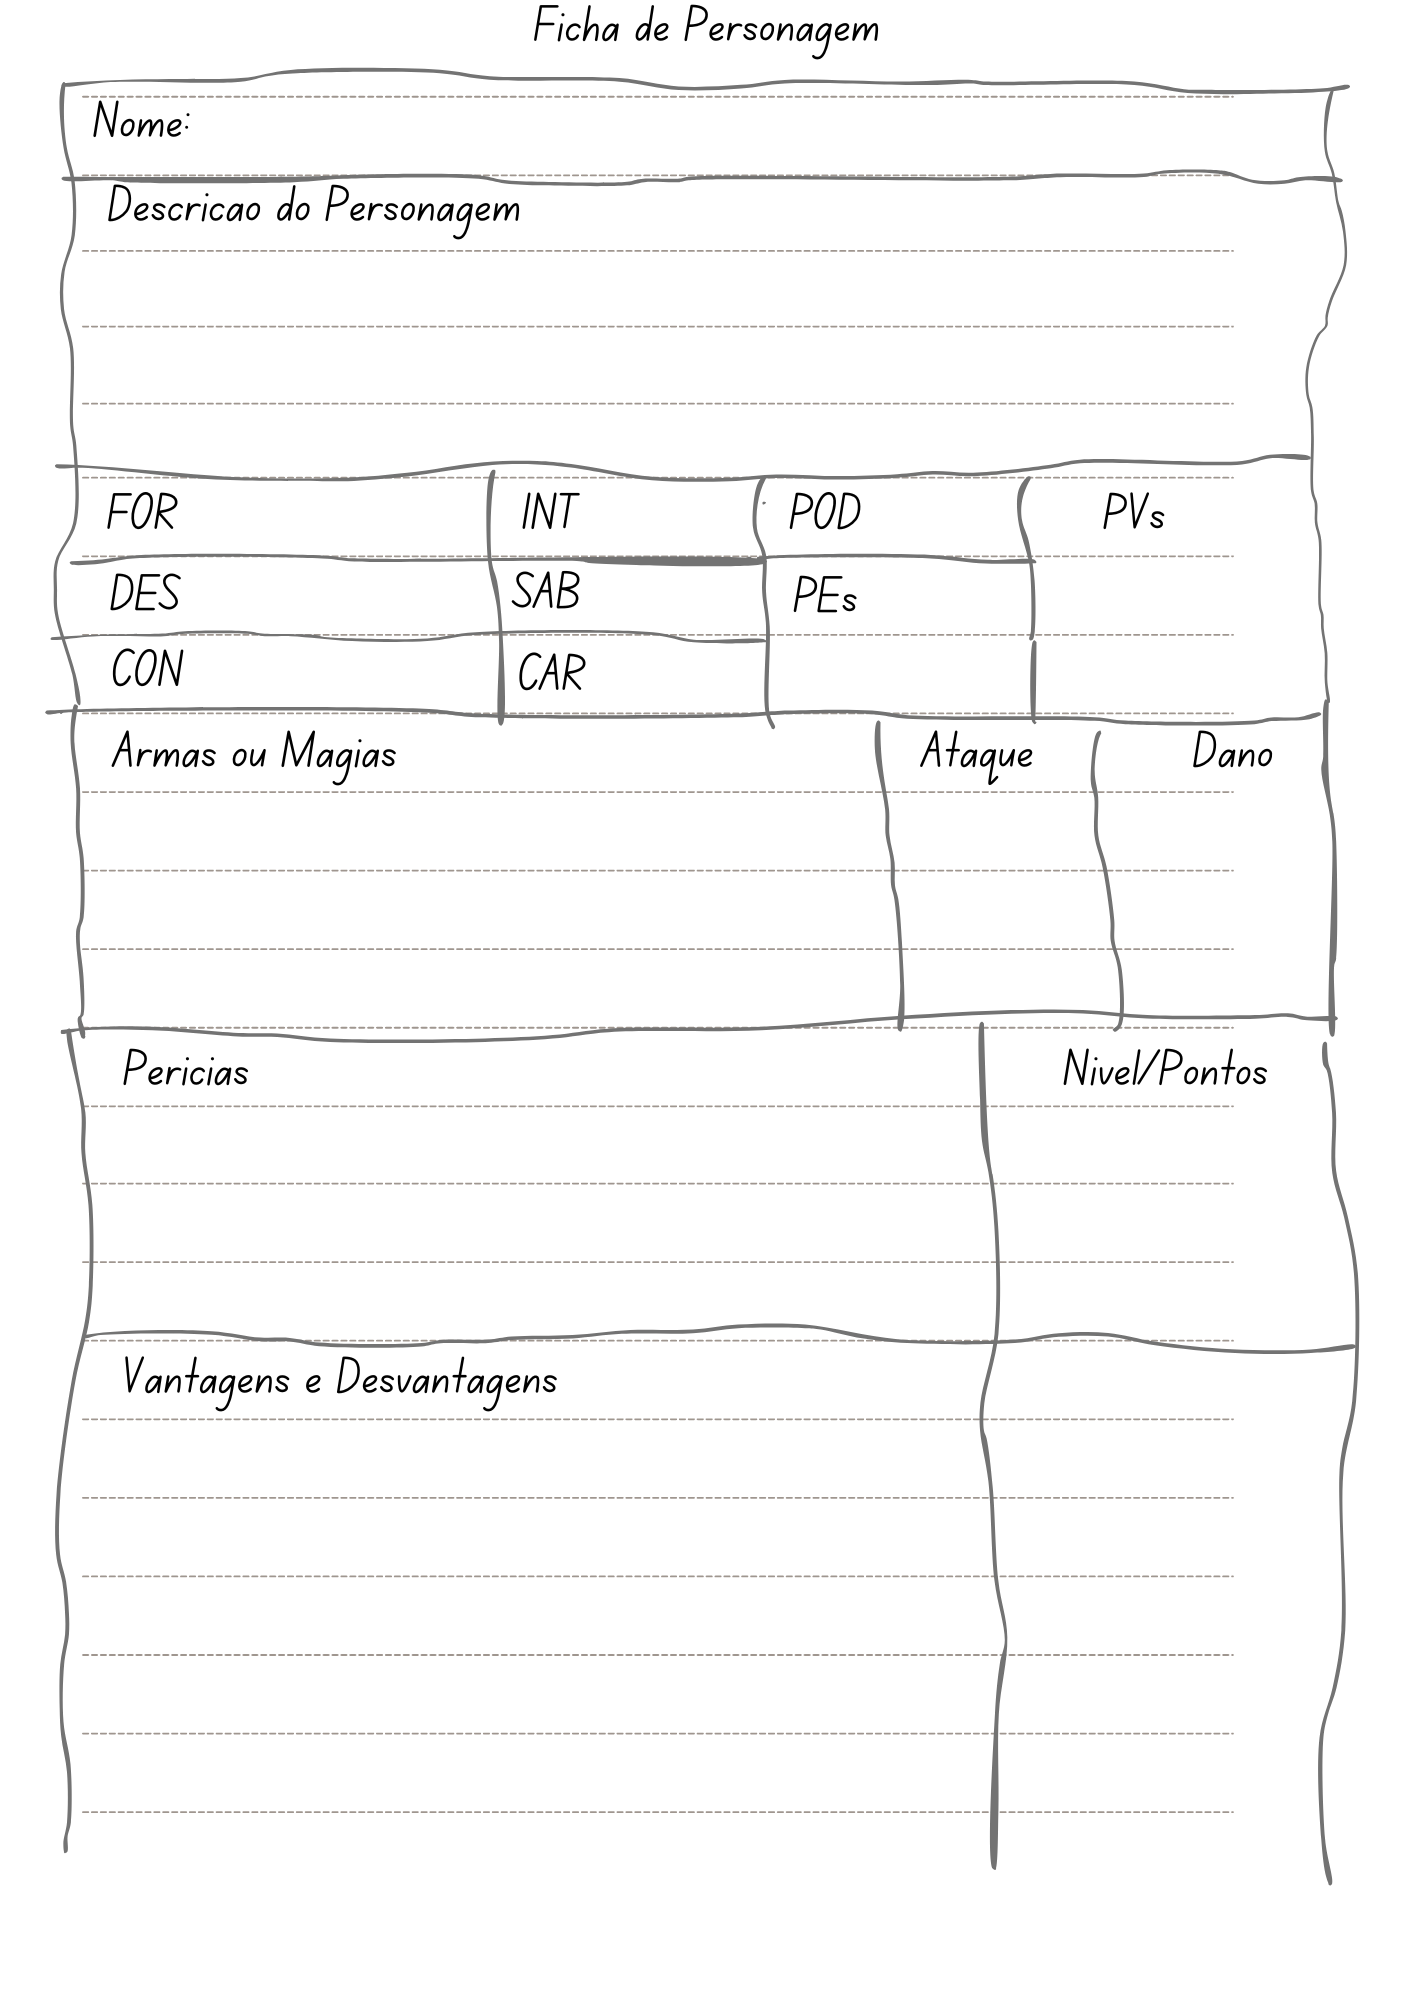
\includegraphics[scale=0.5]{img/fichaManual.png}
	\caption{Exemplo de ficha feita a mão livre.}
	\label{fichaMaoLivre}
\end{figure}

\subsection{\label{subsecAtributos}Atributos}

\subsection{\label{subsecPericias}Perícias}
\subsection{\label{subsecVantagens}Vantagens e Desvantagens}
	\chapter{\label{ch:classes}Classes de Personagem}

Classes são como funções que o personagem exerce/assume durante uma aventura. Assim, ao criar seu personagem, o jogador define qual classe irá interpretar durante a aventura. Destacamos que o Sistema +2d6@IM não obriga o uso das classes, portante os jogadores podem criar seus personagens sem classe.

As seções a seguir apresentam as principais classes do sistema +2d6@IM, mas outras podem ser criadas livremente.


\section{\label{sec:aventMedievais}Classes para aventuras fantásticas}

\subsection*{Arqueiros}
O arqueiro é uma classe de personagem que domina a arte do combate à distância. Com um arco e flecha em mãos, agilidade e conhecimento tático do terreno, fazem do arqueiro um personagem formidável, capaz de lançar com vantagem a partir de locais estratégicos e privilegiados. 

\begin{table}[htb]
	\centering\smaller
	\emph{Inteligências importantes para Arqueiros.}
	\begin{tabu} to \textwidth {|X[c 0.5]|X[1]|X[3]|} \tabucline-
		\textbf{Ordem}	& \textbf{Inteligência}	&	\textbf{Descrição}	\\ \tabucline-
		1º		& \emph{Corporal-cinestésica - Destreza}  	& Confere a capacidade para o manejo de armas a distância.	\\ \tabucline-
		2º		& \emph{Espacial} & Confere a capacidade de reconhecer e escolher bem o terreno onde estiver, seja em combate ou não.\\ \tabucline-
	\end{tabu}
\end{table}

\begin{table}[htb]
	\centering\smaller
	\emph{Equipamentos importantes para Arqueiros.}
	\begin{tabu} to \textwidth {|X[0.5]|X[3]|} \tabucline-
		\textbf{Equipamentos}	&	\textbf{Descrição}	\\ \tabucline-
		\emph{Armaduras}  	& Apenas armaduras leves de material não reflexivo. Metal ou outro material que reflete a luz podem dificultar ações de camuflagem ou furtivas.	\\ \tabucline-
		\emph{Armas} & Preferem arco longo, mas sabem/podem utilizar qualquer tipo de arma a distância como arcos, besta ou dardos. As flechas serão carregadas em uma aljava, com capacidade para 20 a 25 flechas ou virotes.\\ \tabucline-
	\end{tabu}
\end{table}


\subsection*{Bárbaros}
O bárbaro é um guerreiro primitivo e indomável, que canaliza sua fúria nas batalhas. Ligado profundamente aos instintos mais básicos, ele enfrenta seus inimigos com uma ferocidade inigualável. Seu corpo é uma arma que possui grande resistência a golpes e é capaz de infligir danos devastadores. Os bárbaros são conhecidos por sua resistência física e agilidade.

\begin{table}[htb]
	\centering\smaller
	\emph{Inteligências importantes para Bárbaros.} \\
	\begin{tabu} to \textwidth {|X[c 0.5]|X[1]|X[3]|} \tabucline-
		\textbf{Ordem}	& \textbf{Inteligência}	&	\textbf{Descrição}	\\ \tabucline-
		1º		& \emph{Corporal-cinestésica - Força}  	& Confere a capacidade de luta no sentido de causar dano.	\\ \tabucline-
		2º		& \emph{Corporal-cinestésica - Destreza} & Confere a capacidade de esquiva e mobilidade durante combates. \\ \tabucline-
		3º		& \emph{Vitalidade} & Devido a natureza selvagem do bárbaro e sua aptidão ao combate corpo-a-corpo, recomenda-se destinar pontos para Vitalidade, pois a quantidade de vida é proporcional à este atributo.\\ \tabucline-
	\end{tabu}
\end{table}

\begin{table}[htb]
	\centering\smaller
	\emph{Equipamentos importantes para Bárbaros.}
	\begin{tabu} to \textwidth {|X[0.5]|X[3]|} \tabucline-
		\textbf{Equipamentos}	&	\textbf{Descrição}	\\ \tabucline-
		\emph{Armaduras}  	& Apenas armaduras leves para facilitar sua mobilidade.	\\ \tabucline-
		\emph{Armas} & Preferem machados de guerra, mas são capazes de utilizar qualquer tipo de arma.\\ \tabucline-
	\end{tabu}
\end{table}

\subsection*{Clérigos}
O clérigo dedica sua existência ao sagrado e cultiva uma fé inabalável em uma divindade superior existente na história. Este deus concede força moral e poder mágico ao clérigo, que luta incansavelmente contra as hordas do mal e criaturas conspurcadas pelas sombras malignas. Entretanto, clérigos nunca causarão ferimentos graves a outras criaturas, a não ser que tenha certeza de que ela esteja a trabalho das forças do mal.

Além de seus poderes curativos, armas sagradas e magias divinas, o clérigo possui grande sabedoria e conhecimento das escrituras sagradas (do seu deus), sendo, algumas vezes, um tipo de guia espiritual para seu grupo, oferecendo conselhos e apoio em momentos de necessidade.

\begin{table}[htb]
	\centering\smaller
	\emph{Inteligências importantes para Clérigos.} \\
	\begin{tabu} to \textwidth {|X[c 0.5]|X[1]|X[3]|} \tabucline-
		\textbf{Ordem}	& \textbf{Inteligência}	&	\textbf{Descrição}	\\ \tabucline-
		1º		& \emph{Intrapessoal/Existencial}  	& Confere a capacidade de de comunhão espiritual com sua divindade, por onde recebe sua força e magia. 	\\ \tabucline-
		2º		& \emph{Interpessoal} & Confere a capacidade de estabelecer uma forte relação e grande influência em seus seguidores, que o caracteriza como ``guia espiritual''. \\ \tabucline-
		3º		& \emph{Vitalidade} & Devido a natureza combatente do clérigo e seu forte desejo de destruir todo o mal, recomenda-se destinar pontos para Vitalidade, pois a quantidade de vida é proporcional à este atributo.\\ \tabucline-
	\end{tabu}
\end{table}

\begin{table}[htb]
	\centering\smaller
	\emph{Equipamentos importantes para Bárbaros.}
	\begin{tabu} to \textwidth {|X[0.5]|X[3]|} \tabucline-
		\textbf{Equipamentos}	&	\textbf{Descrição}	\\ \tabucline-
		\emph{Armaduras}  	& Qualquer tipo de armadura, mas preferem armaduras pesadas e reluzentes.	\\ \tabucline-
		\emph{Armas} & Apenas as com dano de \emph{concussão}. Devido aos juramentos feitos à divindade e adoção de doutrinas sagradas, clérigos são impedidos de utilizar qualquer arma afiada (que cause cortes ou perfurações), pois nem mesmo a mais infame criatura merece ter seu sangue derramado.\\ \tabucline-
		\emph{Símbolo sagrado} & Clérigos carregam sempre consigo um artefato ou símbolo sagrado, que foi abençoado por seu deus e que funciona como um foco do seu poder mágico. Por exemplo: medalhão, adaga sagrada, pérola negra, etc... \\ \tabucline-
	\end{tabu}
\end{table}

\subsection*{Druida}
Druidas possuem uma profunda conexão com a Natureza, de onde buscam forças, alimentos, medicamentos e até poderes mágicos elementais. Com um profundo respeito e conhecimento pelo mundo natural e suas criaturas, eles possuem a capacidade de convocar os poderes da terra, do ar, do fogo e da água para os auxiliar em suas jornadas. 

Seus poderes mágicos permitem que ele se transforme em animais, comunique-se com plantas e controlem os 4 elementos. Além de suas habilidades mágicas, o druida é um ferrenho defensor da natureza, utilizando suas habilidades para proteger florestas, rios e criaturas selvagens. Muitas vezes, os druidas são vistos como sábios e conselheiros, oferecendo a seus conhecimentos sobre as plantas medicinais e os ciclos da natureza para ajudar aqueles que cruzam seu caminho.

Devido a sua profunda conexão com a Natureza, os druidas sabem que a terra foi ferida, tendo suas entranhas rasgadas para que o metal saísse de suas profundezas, portando, não se permitem usar/vestir nada feito de metal.

\begin{table}[htb]
	\centering\smaller
	\emph{Inteligências importantes para Druidas.} \\
	\begin{tabu} to \textwidth {|X[c 0.5]|X[1]|X[3]|} \tabucline-
		\textbf{Ordem}	& \textbf{Inteligência}	&	\textbf{Descrição}	\\ \tabucline-
		1º		& \emph{Naturalista}  	& Confere conhecimentos da Natureza, suas criaturas, poderes elementais, etc. 	\\ \tabucline-
		2º		& \emph{Espacial} & Confere conhecimento dos lugares e espaços onde há Natureza selvagem. \\ \tabucline-
	\end{tabu}
\end{table}

\begin{table}[htb]
	\centering\smaller
	\emph{Equipamentos importantes para Druidas.}
	\begin{tabu} to \textwidth {|X[0.5]|X[3]|} \tabucline-
		\textbf{Equipamentos}	&	\textbf{Descrição}	\\ \tabucline-
		\emph{Armaduras} & Apenas armaduras e escudos feitos de elementos naturais, como madeira, cipós, etc.	\\ \tabucline-
		\emph{Armas} & Apenas simples como clavas e bastões ou armas fabricadas com galhos, pedras e ossos. \\ \tabucline-
		\emph{Cajado} & Druidas portam sempre um cajado feito nobres elementos naturais, como um majestoso galho cedido pela árvore anciã e ricamente adornado com penugens retiradas de ninhos abandonados. O cajado é um catalisador do poder elemental presente na Natureza, permitindo ao Druida conjurar suas magias. \\ \tabucline-
	\end{tabu}
\end{table}

\subsection*{Bardo}
O bardo é um artista itinerante que utiliza a magia proveniente da arte, da música ou da poesia, para inspirar e influenciar aqueles ao seu redor. Com um instrumento em mãos, ele é capaz de compor canções épicas, contar histórias fascinantes e até mesmo manipular as emoções dos outros. 

A magia do bardo é única, pois ela está intimamente ligada à sua criatividade e à força de suas palavras. Seja acalmando uma criatura selvagem com uma melodia suave ou fortalecendo seus aliados na batalha com uma canção inspiradora, o bardo é um membro valioso em qualquer grupo de aventureiros. Bardos também podem ser ótimos encrenqueiros e grandes sedutores. 

\begin{table}[htb]
	\centering\smaller
	\emph{Inteligências importantes para Bardos.} \\
	\begin{tabu} to \textwidth {|X[c 0.5]|X[1]|X[3]|} \tabucline-
		\textbf{Ordem}	& \textbf{Inteligência}	&	\textbf{Descrição}	\\ \tabucline-
		1º		& \emph{Artística/Musical}  	& Confere habilidades de interpretação, representação, canto, domínio de instrumentos musicais, etc. 	\\ \tabucline-
		2º		& \emph{Interpessoal} & Confere habilidades de interação social, carisma e sedução. \\ \tabucline-
	\end{tabu}
\end{table}

\begin{table}[htb]
	\centering\smaller
	\emph{Equipamentos importantes para Bardos.}
	\begin{tabu} to \textwidth {|X[0.5]|X[3]|} \tabucline-
		\textbf{Equipamentos}	&	\textbf{Descrição}	\\ \tabucline-
		\emph{Armaduras} & Apenas armaduras leves.	\\ \tabucline-
		\emph{Armas} & Armas simples como adagas, rapieiras, espadas curtas ou bestas de mão. \\ \tabucline-
		\emph{Instrumento musical} & Um instrumento como flauta, alaúde, violino, sanfona ou outro qualquer, desde que seja portátil em uma aventura. O instrumento é usado para diversos fins, principalmente para inspirar companheiros de jornada. \\ \tabucline-
	\end{tabu}
\end{table}

\subsection*{Guerreiro}
Guerreiros são pessoas que receberam intenso treinamento militar. Sabem utilizar qualquer equipamentos de combate e também podem ser habilidosos estrategistas ou comandantes. 

Sua coragem inabalável e sua habilidade de liderar inspirem seus aliados, ao mesmo tempo que sua presença intimidante aterroriza os oponentes. Guerreiros são a linha de frente no combate, onde lutam para proteger aqueles que não podem se defender por si mesmos. 

\begin{table}[htb]
	\centering\smaller
	\emph{Inteligências importantes para Guerreiros.} \\
	\begin{tabu} to \textwidth {|X[c 0.5]|X[1]|X[3]|} \tabucline-
		\textbf{Ordem}	& \textbf{Inteligência}	&	\textbf{Descrição}	\\ \tabucline-
		1º		& \emph{Corporal-cinestésica - Força}  	& Confere habilidades de interpretação, representação, canto, domínio de instrumentos musicais, etc. 	\\ \tabucline-
		2º		& \emph{Interpessoal} & Confere habilidades de liderança, comando, intimidação, etc. \\ \tabucline-
		3º 		& \emph{Vitalidade} & Devido a natureza combatente do guerreiro e seus esforços em proteger os mais fracos, recomenda-se destinar pontos para Vitalidade, pois a quantidade de vida é proporcional à este atributo. \\ \tabucline-
	\end{tabu}
\end{table}

\begin{table}[htb]
	\centering\smaller
	\emph{Equipamentos importantes para Guerreiros.}
	\begin{tabu} to \textwidth {|X[0.5]|X[3]|} \tabucline-
		\textbf{Equipamentos}	&	\textbf{Descrição}	\\ \tabucline-
		\emph{Armaduras} & Qualquer armadura.	\\ \tabucline-
		\emph{Armas} & Qualquer arma. \\ \tabucline-
	\end{tabu}
\end{table}

\subsection*{Ladino}
O ladino é um mestre nas artes da infiltração e dissimulação, com uma habilidade ímpar para se mover nas sombras e enganar seus inimigos. É capaz de abrir fechaduras, desarmar armadilhas e se mover silenciosamente por locais perigosos. Além de suas habilidades físicas, muitos ladinos possuem um conhecimento profundo de diversas culturas e línguas, permitindo-lhes se infiltrar em praticamente qualquer sociedade. 

Com sua natureza astuta e calculista, costuma evitar o combate direto, mas ainda assim é um aliado valioso para qualquer grupo de aventureiros, capaz de obter informações cruciais, desviar perigos e realizar missões perigosas.

\begin{table}[htb]
	\centering\smaller
	\emph{Inteligências importantes para Ladinos.} \\
	\begin{tabu} to \textwidth {|X[c 0.5]|X[1]|X[3]|} \tabucline-
		\textbf{Ordem}	& \textbf{Inteligência}	&	\textbf{Descrição}	\\ \tabucline-
		1º		& \emph{Corporal-cinestésica - Destreza}  	& Confere habilidades para o manuseio de ferramentas delicadas e precisas, bem como de movimentar-se de forma sorrateira e imperceptível. 	\\ \tabucline-
		2º		& \emph{Linguística/Verbal} & Confere conhecimentos de diversas línguas e culturas, incluindo dialetos, gírias e jargões do submundo. \\ \tabucline-
	\end{tabu}
\end{table}

\begin{table}[htb]
	\centering\smaller
	\emph{Equipamentos importantes para Ladinos.}
	\begin{tabu} to \textwidth {|X[0.5]|X[3]|} \tabucline-
		\textbf{Equipamentos}	&	\textbf{Descrição}	\\ \tabucline-
		\emph{Armaduras} & Apenas armaduras leves.	\\ \tabucline-
		\emph{Armas} & Armas simples como adagas, rapieiras, espadas curtas ou bestas de mão. \\ \tabucline-
		\emph{Kit de trabalho} & Ladinos costuma andar sempre com sua pequena maleta de utensílios variados, utilizados para arrombar fechaduras, desarmar armadilhas, descobrir códigos de cofres, etc. \\ \tabucline-
	\end{tabu}
\end{table}

\subsection*{Mago}
O mago é um estudioso das forças místicas do universo, sendo capaz de manipular a trama mágica que nos rodeia. São capazes de criar ilusões, manipular e transformar elementos. Devido aos seus longos anos de estudo, possuem profundo conhecimento de linguagens antigas, runas, rituais, etc. 

O mago possui um grimório, onde todos seus feitiços estão meticulosamente registrados, por esse motivo, irá proteger\footnote{Um mago cuidadoso sempre possui uma cópia de seu grimório guardada em local seguro e conhecido apenas por ele.} seu grimório aconteça o que acontecer.

Para conjurar suas magias o mago precisa ter mãos livres (para fazer os sinais que a magia exige), precisa poder falar (para pronunciar as palavras mágicas) e precisa do seu foco arcano, onde concentra a energia da trama mágica que nos rodeia.

\begin{table}[htb]
	\centering\smaller
	\emph{Inteligências importantes para Magos.} \\
	\begin{tabu} to \textwidth {|X[c 0.5]|X[1]|X[3]|} \tabucline-
		\textbf{Ordem}	& \textbf{Inteligência}	&	\textbf{Descrição}	\\ \tabucline-
		1º		& \emph{Linguística/Verbal}  	& Confere habilidades de compreender e utilizar diversos idiomas, inclusive mágicos. 	\\ \tabucline-
		2º		& \emph{Lógico/Matemática} & Confere habilidades de compreender e manipular as complexas equações arcanas.\\ \tabucline-
	\end{tabu}
\end{table}

\begin{table}[htb]
	\centering\smaller
	\emph{Equipamentos importantes para Magos.}
	\begin{tabu} to \textwidth {|X[0.5]|X[3]|} \tabucline-
		\textbf{Equipamentos}	&	\textbf{Descrição}	\\ \tabucline-
		\emph{Grimório} & Livro com o registro de todas as magias que o mago conhece.	\\ \tabucline-
		\emph{Foco arcano} & É um artefato que concentra seu poder mágico, podendo ser um Cajado, Varinha, Orbe, Amuletos ou Talismãs. \\ \tabucline-
		\emph{Armadura} & Não usam armaduras porque atrapalham seus movimentos para conjurar magias. \\ \tabucline-
		\emph{Armas} & Apenas armas simples. \\ \tabucline-
	\end{tabu}
\end{table}


\subsection*{Paladino}
O paladino é um guerreiro sagrado, imbuído de um forte senso de justiça e honra. Ele é um defensor incansável dos fracos e oprimidos, combatendo as forças do mal com uma espada na mão e uma fé inabalável no coração. 

A força do paladino reside não apenas em sua proeza física, mas também em sua conexão com uma força superior, que lhe concede poderes divinos e a capacidade de curar feridas e abençoar seus aliados. Os paladinos são conhecidos por sua coragem inabalável, sua lealdade e seu compromisso com um código de honra rígido. 

Com sua armadura brilhante e sua aura de santidade, o paladino inspira confiança e esperança em todos aqueles que cruzam seu caminho.

\begin{table}[htb]
	\centering\smaller
	\emph{Inteligências importantes para Paladinos.} \\
	\begin{tabu} to \textwidth {|X[c 0.5]|X[1]|X[3]|} \tabucline-
		\textbf{Ordem}	& \textbf{Inteligência}	&	\textbf{Descrição}	\\ \tabucline-
		1º		& \emph{Corporal-cinestésica (Força)} & Confere a força para manusear sua espada contra as forças do mal. \\ \tabucline-
		2º		& \emph{Intrapessoal/Existencial}  	& Confere a conexão divina para suas magias de cura e proteção. 	\\ \tabucline-
	\end{tabu}
\end{table}

\begin{table}[htb]
	\centering\smaller
	\emph{Equipamentos importantes para Paladinos.}
	\begin{tabu} to \textwidth {|X[0.5]|X[3]|} \tabucline-
		\textbf{Equipamentos}	&	\textbf{Descrição}	\\ \tabucline-
		\emph{Armaduras} & Qualquer tipo de armadura (normalmente reluzente e com símbolos sagrados).	\\ \tabucline-
		\emph{Armas} & Qualquer tipo de arma, preferindo as espadas longas ou bastarda. \\ \tabucline-
	\end{tabu}
\end{table}


\subsection*{Rastreador}
Rastreadores são exploradores experientes, conhecem profundamente a natureza e o comportamento dos animais. Com uma percepção aguçada e habilidades de sobrevivência excepcionais, eles navegam por terras selvagens e perigosas com facilidade.

São capazes de rastrear suas presas por longas distâncias e emboscar seus inimigos com muita precisão. Possuem também um profundo conhecimento das plantas, dos animais e dos espíritos da natureza, aproveitando os recursos naturais para sobreviver. 

\begin{table}[htb]
	\centering\smaller
	\emph{Inteligências importantes para Rastreadores.} \\
	\begin{tabu} to \textwidth {|X[c 0.5]|X[1]|X[3]|} \tabucline-
		\textbf{Ordem}	& \textbf{Inteligência}	&	\textbf{Descrição}	\\ \tabucline-
		1º		& \emph{Espacial}  	& Confere habilidades de compreensão e reconhecimento do espaço em que está, bem como de localização. 	\\ \tabucline-
		2º		& \emph{Naturalista} & Confere o conhecimento da natureza. Consegue identificar pegadas de animais, reconhecer plantas, encontrar fontes de água pura, etc. \\ \tabucline-
	\end{tabu}
\end{table}

\begin{table}[htb]
	\centering\smaller
	\emph{Equipamentos importantes para Rastreadores.}
	\begin{tabu} to \textwidth {|X[0.5]|X[3]|} \tabucline-
		\textbf{Equipamentos}	&	\textbf{Descrição}	\\ \tabucline-
		\emph{Armaduras} & Somente as leves e naturais.	\\ \tabucline-
		\emph{Armas} & Qualquer arma comum. \\ \tabucline-
	\end{tabu}
\end{table}


%
%\subsection*{generico}
%texto aqui
%
%\begin{table}[htb]
%	\centering\smaller
%	\emph{Inteligências importantes para ???.} \\
%	\begin{tabu} to \textwidth {|X[c 0.5]|X[1]|X[3]|} \tabucline-
%		\textbf{Ordem}	& \textbf{Inteligência}	&	\textbf{Descrição}	\\ \tabucline-
%		1º		& \emph{???}  	& Confere habilidades ???. 	\\ \tabucline-
%		2º		& \emph{???} & Confere ???? \\ \tabucline-
%	\end{tabu}
%\end{table}
%
%\begin{table}[htb]
%	\centering\smaller
%	\emph{Equipamentos importantes para ???.}
%	\begin{tabu} to \textwidth {|X[0.5]|X[3]|} \tabucline-
%		\textbf{Equipamentos}	&	\textbf{Descrição}	\\ \tabucline-
%		\emph{Armaduras} & ????.	\\ \tabucline-
%		\emph{Armas} & ????. \\ \tabucline-
%		\emph{?????} & ????. \\ \tabucline-
%	\end{tabu}
%\end{table}
%

%
%\subsection*{\textcolor{red}{Alquimistas}}
%Os alquimistas são estudiosos que unem ciência e natureza, buscando a transmutação matéria e energia. Na busca por dominar a alquimia, estão constantemente procurando saber mais sobre os elementos e da natureza.
%
%São capazes de criar poções e elixires, que podem aumentar a força, curar ferimentos 
%
%Utilizando seus instrumentos 
%
%Inteligências recomendadas:
%\begin{itemize}
%	\item \textbf{Principal}: Lógico-Matemática
%	\item \textbf{Secundária}: Naturalista
%\end{itemize}
%
%
%
%\subsection*{\textcolor{red}{Artífice}}
%Inteligências 
%\begin{itemize}
%	\item \textbf{Principal}: Artística/Musical
%	\item \textbf{Secundária}: Lógico-matemática
%\end{itemize}
%
%\subsection*{Monge}
%Inteligências 
%\begin{itemize}
%	\item \textbf{Principal}: Corporal-cinestésica - Destreza
%	\item \textbf{Secundária}: Intrapessoal/Existencial
%\end{itemize}
%
%\subsection*{Psiônicos}
%Inteligências 
%\begin{itemize}
%	\item \textbf{Principal}: Interpessoal
%	\item \textbf{Secundária}: Linguística/Verbal
%\end{itemize}
%

%
%\section{\label{sec:aventModernas}Aventuras Modernas}
	\chapter{\label{ch:jogando}Jogando com +2d6@IM}


\section{\label{sec:testes}Jogadas de teste}

\section{\label{sec:combate}Combates}

\section{\label{sec:descanso}Descanso}
São os jogadores que informam ao Mestre que irão fazer um descanso e para isso, precisam monitorar a quantidade de energia que seu personagem ainda tem e o Mestre precisa manter os jogadores informados sobre o tempo no jogo.
	\chapter{\label{ch:magia}Magia Antiga}
	\chapter{\label{ch:equipamentos}Equipamentos do Aventureiro}



\section{\label{sec:armas}Armas}


\subsection{\label{sec:armasCorpoAcorpo}Armas corpo-a-corpo}

Cortante: Espadas, machados, facas. Causam ferimentos profundos por meio de cortes.
Curta distância: Facas, adagas, martelos de guerra. Utilizadas em combate corpo a corpo.
Média distância: Espadas, machados de mão. Também utilizadas em combate corpo a corpo, mas com maior alcance.
Perfurante: Lanças, espadas longas
Contundente: Maças, martelos de guerra. Infligem danos por impacto, causando contusões e fraturas.



\subsection{\label{sec:armasDistancia}Armas a distância}
Longa distância: Arcos, bestas, lançadores de dardos. Utilizadas para atacar inimigos a distância.


\subsection{\label{sec:armasDistancia}Armas naturais/druídicas}
Longa distância: Arcos, bestas, lançadores de dardos. Utilizadas para atacar inimigos a distância.
funda
adaga de obsidiana
adaga de osso
machado de osso de mandíbula


\section{Escudos e Armaduras}

\subsubsection{\label{sec:armadLeves}Armaduras Leves}
Armadura acolchoada 	5 TO 	+1 	+8 	0 	5Kg
Corselete de couro 	10 TO 	+2 	+6 	0 	7Kg
Couro batido 	25 TO 	+3 	+5 	-1 	10Kg
Camisa de cota de Malha 	100 TO 	+4 	+4 	-2 	12Kg
Couro Cristalino 	4.500 TO 	+3 	5 	0 	10Kg

\subsubsection{\label{sec:armadPesada}Armaduras Pesada}
Gibão de peles 	15 TO 	+3 	+4 	-2 	12Kg
Brunea 	50 TO 	+4 	+3 	-3 	15Kg
Cota de malha 	150 TO 	+5 	+2 	-3 	20Kg
Couraça 	200 TO 	+5 		-4 	15Kg
Armadura de Gladiador 	200 TO 	+5 	+2 	-5 	15Kg
Couraça de Bronze 	500 TO 	+4 	+4 	-4 	12Kg


\subsubsection{\label{sec:escudos}Escudos}
Escudo leve 	5 TO 	+1 	--- 	-1 	3Kg
Escudo pesado 	15 TO 	+2 	--- 	-2 	7Kg
Escudo de corpo 	50 TO 	+4 	--- 	-5 	15Kg 


\subsubsection{Ferramentas}
Ladino : http://sonhonautarpg.blogspot.com/2017/05/novo-item-ferramentas-de-ladrao.html
	\chapter{\label{ch:mestre}Área do Mestre}
	
	\backmatter
	% bibliography, glossary and index would go here.
	
	\postextual
	\apendices
	\chapter{\label{apendiceFichas}Apêndice I - Exemplos de Ficha de Personagem}
	\chapter{\label{apendicePericias}Lista de Perícias}

As perícias sugeridas nessa listagem a seguir são as mais comuns em Mesas de RPG. Os jogadores de uma mesa podem criar novas perícias desde que todos estejam em comum acordo. Por exemplo: partindo de \emph{Resistência à venenos} pode-se criar \emph{Resistência ao frio} e \emph{Resistência ao fogo}. 

Esta listagem organiza as perícias em função da sua aplicação e dos tipos de atributos.

\section{\label{sec:perArmas}Perícias com armas}
\begin{itemize}
	\item Armas comuns (FOR ou DES): Você sabe utilizar armas comuns como facas, machadinhas, porretes, facão machete, funda, besta de mão, arco curto, etc.
	\item Armas profissionais corpo-a-corpo (FOR): Você sabe usar armas profissionais de combate corpo-a-corpo, como espadas de todos os tipos 	
	\item Armas profissionais à distância (DES): Você sabe usar armas profissionais à distância como arcos, arma de fogo, arma de energia, lanças, etc.
	\item Artilharia (INT): Você sabe operar artilharia militar pesada, artilharia antiaérea, etc.
	\item Armadilhas (DES): Você consegue identificar e desarmar armadilhas não mágicas.
\end{itemize}

\section{\label{sec:perFisicos}Perícias baseadas de atributos físicos}
Perícias relativas à Força, Destreza ou Constituição:
\begin{itemize}
	\item Acrobacia (DES): Você sabe executar saltos mortais ou acrobáticos, estrelas, salto em distância ou altura, equilibrismo, etc.
	\item Arte da Fuga (DES): Você possui habilidades para escapar de amarras, correntes ou algemas, rastejar por espaços apertados,etc.
	\item Arremessar (DES): Você sabe lançar pequenos objetos usando apenas as mãos (pedras, dardos, etc).
	\item Arrombamento (DES): Você tem tem conhecimento para abrir fechaduras mecânicas de portas, cofres, prédios, etc.
	\item Artes Marciais (DES): Você conhece artes marciais. Dependendo do tipo de aventura, pode-se criar uma perícia específica para cada tipo de arte marcial (Judô, Karatê, Jiu-jitsu, etc).
	\item Atletismo (FOR): Você possui treinamento de força e consegue executar tarefas que exijam força muscular como levantar objetos pesados, carregar grandes cargas, etc.
	\item Cavalgar (DES): Você sabe andar a cavalo (ou outro animal de carga equivalente).
	\item Controle da Respiração (CON): Você conhece técnicas para prender ou controlar a respiração por alguns minutos. Como sugestão, o tempo limite poderia ser 1d6 + pontos usados para compra da vantagem.
	\item Escalar (FOR ou DES): Você conhece técnicas para escalar superfícies íngremes a uma velocidade igual ao Deslocamento/4.
	\item Esconder-se (DES): Você tem habilidade para esconder-se com facilidade. Em combate, se sua localização é conhecida, é preciso "trocar de esconderijo".
	\item Furtividade (DES): Você tem a habilidade de aproximar-se sem ser notado, andar silenciosamente, passar despercebido, etc.
	\item Natação (FOR ou DES): Você sabe nadar e mergulhar.
	\item Punga (DES): Você desenvolveu habilidades para roubar pessoas sem ser percebido (roubar carteira, celular, documentos).
	\item Resistência à venenos (CON): Você é resistente à venenos, recebendo apenas a metade do dano causado pelo veneno inoculado no seu corpo.
	\item Tolerância (CON): Possui uma maior capacidade de resistir dor, fadiga, fome e sede.
\end{itemize}

\section{\label{sec:perMentais}Perícias de atributos mentais}
Lista com Perícias relativas à Inteligência, Sabedoria ou Carisma.

\subsubsection*{Inteligência}
\begin{itemize}
	\item Administração (INT): Você tem conhecimentos sobre gerência, liderança, atividades corporativas, etc.
	\item Cartografia (INT): Você sabe interpretar e criar mapas, bem como mapear locais desconhecidos, etc.
	\item Ciência Forense (INT): Você tem conhecimentos para descobrir sobre causas de mortes, sabe fazer autópsias, etc.
	\item Ciências Ocultas (INT): Você tem conhecimento sobre práticas de ocultismo e outras ciências não oficiais, que envolvem temas tabus e proibidos como magia, demonologia, estudo dos espíritos, etc.
	\item Cibernética (INT): Você tem conhecimento de sistemas cibernéticos variados.
	\item Estratégia Militar (INT): Você tem conhecimento de táticas militares, capaz de reconhecer táticas militares do inimigo, descobrir pontos fracos, estabelecer táticas de combate eficazes.
	\item Explosivos (INT): Você sabe armar e desarmar explosivos, criar bombas, etc.
	\item Falsificação (INT): Você tem habilidades para falsificar documentos, objetos de arte, dinheiro, etc.
	\item Hacking (INT): Você sabe criar programas, invadir sistemas, criar vírus de computador, tomar controle de redes de telecomunicações, etc.
	\item História (INT): Você tem conhecimento de fatos históricos locais ou globais, conhece culturas primitivas e contemporâneas do mundo onde a aventura acontece.	
	\item Medicina (INT): Você conhecimentos de medicina, realizar operações, tratar ferimentos e doenças, etc.
	\item Metalurgia (INT): Você sabe criar e reparar coisas feitas de metal, como armas, armaduras, equipamentos, etc.
	\item Mitos de Cthulhu (INT): Você tem conhecimento dos inomináveis horrores cósmicos.
	\item Ofícios em <área> (INT): perícia genérica para representar algum tipo de habilidade técnica como artesanato, escultura, ferraria, criação de animais, agricultura, joalheria, etc.
	\item Pilotar Veículos <tipo> (INT): Você sabe pilotar veículos de algum tipo. O tipo pode ser: terrestre, aquáticos, aéreos, espaciais.
	\item Veterinária (INT): Você sabe tratar ferimentos e doenças de animais, conhecimento de biologia animal.	
\end{itemize}

\subsubsection*{Carisma}
\begin{itemize}
	\item Atuação (CAR): Você sabe interpretar papéis, atuar artisticamente com dança, música, contando histórias, etc.
	\item Disfarces(CAR): Você sabe como se disfarçar, como criar disfarces, etc.
	\item Diplomacia (CAR): Você possui habilidades para criar relações com outros povos e culturas.
	\item Enganação (CAR): Você tem habilidades para enganar/iludir as outras pessoas.
	\item Hipnose (CAR): Você conhece técnicas para afetar a mente de uma pessoa e torná-la mais fácil de ser manipulada.
	\item Intimidação (CAR): Você sabe influenciar/convencer alguém por meio de ameaças, ações hostis, etc.
	\item Obter informações (CAR): Você tem a habilidade de obter informações valiosas de fontes inesperadas.
	\item Persuasão (CAR): Você tem habilidade de influenciar/convencer alguém por meio da conversa delicada e agradável, com tato. 
	\item Sedução (CAR): Você tem habilidades e conhece técnicas de sedução.
\end{itemize}

\subsubsection*{Sabedoria}
\begin{itemize}
	\item Curanderismo (SAB): Você sabe usar plantas e ervas para preparar remédios e curativos.
	\item Intuição (SAB): Você tem um sentido extra, que ajuda a não ser enganado e a perceber situações estranhas.
	\item Natureza (SAB): Você tem conhecimento sobre a Natureza e os seres que nela habitam.
	\item Navegação (SAB): Você sabe conduzir embarcações e se orientar em alto mar, etc.
	\item Percepção (SAB): Você tem mais facilidade em perceber situações e eventos.
	\item Poções (SAB): Você sabe identificar e criar poções variadas.
	\item Procurar (SAB): habilidade de vasculhar com atenção, notar pequenas diferenças, muito útil para investigadores.
	\item Rastrear (SAB): Você saber rastrear, seguir rastros, perseguir uma presa ou pessoa.
	\item Vontade (SAB): Você tem controle sobre sua Força de Vontade e pode resistir ao medo, à hipnose, poderes mentais, etc.
	\item Sobrevivência (SAB): Você tem habilidades de sobreviver em lugares selvagens, encontrar abrigo, caçar, conseguir alimento, reconhecer plantas venenosas, encontrar a direção, etc.
\end{itemize}
	
\subsubsection*{Inteligência ou Sabedoria}
\begin{itemize}
	\item Exorcismo (INT/SAB): Você sabe realizar rituais de exorcismo.
	\item Investigação (INT/SAB): Você sabe avaliar crimes/situações para reunir pistas, evidências, deduzir, etc.
	\item Perceber Magia (INT/SAB): Você tem conhecimento para identificar presença de magia em ambientes, objetos, lugares, etc.
	\item Religião (INT/SAB): Você tem conhecimento teológico, de história das religiões, da ritualística, etc.
	\item Venenos (INT/SAB): Você sabe saber criar, usar, identificar e neutralizar venenos.
\end{itemize}


	\chapter{\label{apendiceVantagensDesvantagens}Lista Vantagens e Desvantagens}

atributos podem ser especificos, qualquer atributo ou especial. Especial significa que não é preciso atributo

\section*{Vantagens}
As vantagens listadas possuem Nome, atributo relacionado (sempre entre parêntesis) e uma explicação. Logo abaixo uma tabela com:
\begin{itemize}
	\item \textbf{Custo} - informando o custo para compra da vantagem. O custo poderá ser único ou variado, nos casos de vantagem com níveis diferentes.
	\item \textbf{Ativação} - informa quantos Pontos de Energia são necessários para ativar a vantagem. O traço (-) é usado para informar que a vantagem não usa PEs, ou seja, está sempre ativada.
	\item \textbf{Descrição} - informa o que muda quando com a vantagem.
\end{itemize}


\begin{small}

\textbf{Absorção de Dano (CON)}: O personagem absorve instantaneamente uma quantidade do dano sofrido. \\
\begin{tabu}{|X[c]|X[c]|X[3]|} \tabucline-
	\textbf{Custo} 	& \textbf{Ativação}	&	\textbf{Descrição} \\ \tabucline-		
	1 ponto	& 2 PEs &	Absorve 3 de dano \\ \tabucline-
	2 ponto	& 2 PEs &	Absorve 6 de dano \\ \tabucline-
	3 ponto	& 2 PEs &	Absorve 9 de dano \\ \tabucline-
	4 ponto	& 2 PEs &	Absorve 12 de dano \\ \tabucline-
	5 ponto	& 2 PEs &	Absorve 15 de dano \\ \tabucline-
\end{tabu}


\textbf{Adaptabilidade Cultural (INT)}: O personagem consegue se adaptar a ambientes culturais ou alienígenas totalmente diferentes do que está acostumado. 

\begin{tabu}{|X[c]|X[c]|X[3]|} \tabucline-
		\textbf{Custo} 	& \textbf{Ativação}	&	\textbf{Descrição} \\ \tabucline-		
		1 ponto	& - &	Ganha +2 em testes de Carisma. \\ \tabucline-
\end{tabu}
	

\textbf{Aliados (CAR)}: Personagem tem aliados (PdMs), que estarão à disposição do personagem. A quantidade máxima de aliados é 3. \\
\begin{tabu}{|X[c]|X[c]|X[3]|} \tabucline-
		\textbf{Custo} 	& \textbf{Ativação}	&	\textbf{Descrição} \\ \tabucline-		
		1 ponto	& - &	Tem 1 aliado \\ \tabucline-
		2 ponto	& - &	Tem 2 aliados \\ \tabucline-
		3 ponto	& - &	Tem 3 aliados \\ \tabucline-
	\end{tabu}


\textbf{Anfíbio (CON)}: Personagem tem capacidades de anfíbio. Não consome PEs.

	\begin{tabu}{|X[c]|X[c]|X[3]|} \tabucline-
	\textbf{Custo} 			& \textbf{Ativação}		&	\textbf{Descrição} \\ \tabucline-
		2 pontos			&		- 				&	Pode respirar embaixo da água. \\ \tabucline-
	\end{tabu}


\textbf{Aparência encantadora (CAR)}: Personagem possui uma beleza incomum. 

	\begin{tabu}{|X[c]|X[c]|X[3 c]|} \tabucline-
		\textbf{Custo} 	& \textbf{Ativação}	&	\textbf{Descrição} \\ \tabucline-
		1 ponto					&	- 							&	Ganha +2 em testes sociais. \\ \tabucline-
		2 ponto					&	-							&	Ganha +4 em testes sociais. \\ \tabucline-
		3 ponto					&	-							&	Ganha +6 em testes sociais. \\ \tabucline-
	\end{tabu}


\textbf{Ataque Especial (Qualquer atributos)}: O personagem possui um ataque especial que garante dano extra.

	\begin{tabu}{|X[c]|X[c]|X[3]|} \tabucline-
	\textbf{Custo} 	& \textbf{Ativação}	&	\textbf{Descrição} \\ \tabucline-
	1 ponto		&	1 PEs. 			& Ganha +1d6 de dano extra em um alvo. \\ \tabucline-
	2 pontos	&	2 PEs 			& Ganha +2d6 de dano extra em um alvo ou +1d6 em dois alvos. \\ \tabucline-
	3 pontos	&	3 PEs 			& Ganha +3d6 de dano extra em um alvo, ou +2d6 em dois alvos ou +1d6 em três alvos.\\ \tabucline-
	4 pontos	&	4 PEs 			& Ganha +4d6 de dano extra em um alvo, ou +3d6 em dois alvos ou +2d6 em três alvos. \\ \tabucline-
	5 pontos	&	5 PEs 			& Ganha +5d6 de dano extra em um alvo, ou +4d6 de dano extra em dois alvos ou +3d6 em três alvos. \\ \tabucline-
	\end{tabu}


\textbf{Aumento de velocidade (DES)}: Personagem tem um corpo super-veloz.

	\begin{tabu}{|X[c]|X[c]|X[3]|} \tabucline-
		\textbf{Custo} 		& \textbf{Ativação}		&	\textbf{Descrição} \\ \tabucline-
		3 pontos			&	4 PEs				&	Ganha DES+10, durante 10 minutos. \\ \hline
	\end{tabu}



\textbf{Aumento da densidade (PODER)}: Personagem pode aumentar a densidade do seu corpo temporariamente, ganhando Redução de Dano extra.

	\begin{tabu}{|X[c]|X[c]|X[3]|} \tabucline-
	\textbf{Custo} 	& \textbf{Ativação}	&	\textbf{Descrição} \\ \tabucline-
	3 pontos				&	3 PEs 						&	Ganha RD = 15, durante 10 minutos. \\ \tabucline-
	\end{tabu}



\textbf{Braços Cibernéticos (DES ou FOR)}: Personagem possui implantes cibernéticos nos braços, que aumentam a força e destreza. Os implantes precisam de  recarga (com eletricidade, carvão, plutônio, etc) e manutenção periódicas (definir a periodicidade com o Mestre).

	\begin{tabu}{|X[c]|X[c]|X[3]|} \tabucline-
	\textbf{Custo} 	& \textbf{Ativação}	&	\textbf{Descrição} \\ \tabucline-
	\multirow{2}{*}{4 pontos}	& 	2 PEs			& Ganha +4 em FOR e DES por 10 minutos . \\ \tabucline{2-3}
								& 	4 PEs			& Causa uma descarga elétrica ao tocar o alvo com 2d6 de dano \\ \tabucline-
	\end{tabu}

\textbf{Camaleão (CAR)}: De alguma forma, o personagem possui a capacidade de mudar sua forma física, clonando a aparência de um humanoide (pessoa ou criatura com forma humana). O personagem pode gastar mais PEs para aumentar o tempo da clonagem até o máximo de 60 minutos. Atributos, perícias, vantagens e desvantagens não são clonados.\\
\begin{tabu}{|X[c]|X[c]|X[3]|} \tabucline-
	\textbf{Custo} 	& \textbf{Ativação}	&	\textbf{Descrição} \\ \tabucline-
	3	& 	3 PEs			& Clona a aparência um humanoide que o personagem já tenha visto por 10 minutos. Ganha +4 em Carisma em testes sociais quando estiver usando a aparência de outra pessoa. \\ \tabucline-
	5	& 	4 PEs			& Clona um humanoide famoso na história, que o personagem já tenha visto por 10 minutos. Ganha +6 em testes sociais quando estiver usando a aparência do famoso. Definir com o Mestre quem são os famosos conhecidos.\\ \tabucline-
\end{tabu}


\textbf{Carga Extra (FOR)}: Personagem possui habilidade para carregar mais carga. Carga Extra não aumenta dano.

	\begin{tabu}{|X[c]|X[c]|X[3]|} \tabucline-
		\textbf{Custo} 	& \textbf{Ativação}	&	\textbf{Descrição} \\ \tabucline-
		2	& 	-			& Ganha FOR+3 para cálculo de carga que poder carregar. \\ \tabucline-
	\end{tabu}


\textbf{Corajoso (INT)}: Personagem é muito corajoso.

	\begin{tabu}{|X[c]|X[c]|X[3]|} \tabucline-
		\textbf{Custo} 	& \textbf{Ativação}	&	\textbf{Descrição} \\ \tabucline-
		1	& 	-			& Ganha +2 em testes de medo ou insanidade. \\ \tabucline-
		2	& 	-			& Ganha +4 em testes de medo ou insanidade. \\ \tabucline-
		3	& 	-			& Ganha +6 em testes de medo ou insanidade. \\ \tabucline-
		4	& 	-			& Ganha +8 em testes de medo ou insanidade. \\ \tabucline-
		5	& 	-			& Ganha +10 em testes de medo ou insanidade. \\ \tabucline-
	\end{tabu}


\textbf{Corpo de Água (CON)}: Por algum motivo o corpo do personagem é feito de água e tem forma física maleável. Se chegar a 0 PVs, personagem morre e o corpo se dissolve. 

	\begin{tabu}{|X[c]|X[c]|X[3]|} \tabucline-
		\textbf{Custo} 	& \textbf{Ativação}	&	\textbf{Descrição} \\ \tabucline-
		\multirow{2}{*}{5}	& 	-	& Ganha RD=5 e tem forma física completamente maleável. \\ \tabucline{2-3}
							& 	-	& Usando DES pode tentar envolver alvo com o corpo, causando 2d6+3 de dano por afogamento a cada rodada. \\ \tabucline-
	\end{tabu}


\textbf{Corpo de Ar (CON)}: Por algum motivo o corpo do personagem é feito de ar e tem forma física maleável. Se chegar a 0 PVs, personagem morre com o corpo dissipando no ar. 

	\begin{tabu}{|X[c]|X[c]|X[3]|} \tabucline-
	\textbf{Custo} 	& \textbf{Ativação}	&	\textbf{Descrição} \\ \tabucline-
	\multirow{2}{*}{5}	& 	-	& Recebe 1d6 de dano extra por ataques de energia (fogo, eletricidade, etc). Ataques tipo ventania podem ser feitos a 10m de distância do alvo e causam dano de Força.\\ \tabucline{2-3}
						& 	2	& Pode voar até 60 km/h por 10 minutos. \\ \tabucline-
	\end{tabu}


\textbf{Corpo de Fogo (CON)}: Por algum motivo o corpo do personagem é feito de fogo e tem forma física maleável. Se chegar a 0 PVs, personagem morre com o corpo desfaz em fumaça.

	\begin{tabu}{|X[c]|X[c]|X[3]|} \tabucline-
		\textbf{Custo} 	& \textbf{Ativação}	&	\textbf{Descrição} \\ \tabucline-
		\multirow{3}{*}{5}	& 	-	& Recebe 1d6 de dano extra por ataques com água ou gelo. \\ \tabucline{2-3}
		& 	2	& Pode voar a um Deslocamento 36 km/h. \\ \tabucline{2-3}
		&	3	&	Solta um raio de fogo a até 10 metros que causa 2d6+3 de dano.
		\\ \tabucline-
	\end{tabu}


fogo
O corpo do personagem é feito de fogo. Forma maleável. 
Seu toque causa 2d6 extras de dano de fogo. 
Sofre 1d6 de dano extra sempre que sofrer ataque com água ou gelo. Não sofre penalidades por ferimentos, mas pode ter membros amputados. 

Gastando 2 PE pode esticar um dos membros a até 3 metros. Se chegar a 0 PVs morre, com o corpo dissolvendo. 

Ataques causam dano igual ao dano relativo a
FOR, porém podem ser feitos a até 3 metros de distância. 

Gastando 2 PE pode esticar um dos membros a até 3 metros.  Ataques causam dano igual ao dano relativo a
FOR, porém podem ser feitos a até 3 metros de distância. Pode voar a um Deslocamento
de 10 m/s ou 36km/hora. Solta um raio de fogo a até 10 metros que causa 2d6+3 de
dano.
Corpo de Gelo (CON)
5 pontos: O corpo do personagem é feito de gelo. Ganha armadura natural de RD
5. Não sofre penalidades por ferimentos,mas pode ter membros amputados. Toque
causa 1d6 de dano extra de gelo. Gastando 2 PE pode esticar um dos membros a até 3
metros. Se chegar a 0 PVs morre, com o corpo dissolvendo. Ataques causam dano igual
ao dano relativo a FOR, porém podem ser feitos a até 3 metros de distância. Solta um
raio de gelo a até 10 metros que causa 2d6+3 de dano.

\textbf{Corpo de Metal (CON)}:
5 pontos: O corpo do personagem é feito de metal. Ganha armadura natural de
RD 10. Imune a dano por projéteis, se o total de dano for menor que 20. Não sofre
penalidades por ferimentos,mas pode ter membros amputados. Causa 1d6+FOR+4 de
dano em ataques corporais. Se chegar a 0 PVs morre, com o corpo dissolvendo. O peso
normal aumenta em 200 kg.

\textbf{Corpo de Terra (CON)}:
5 pontos: O corpo do personagem é feito de terra. Ganha armadura natural de
RD 10. Não sofre penalidades por ferimentos,mas pode ter membros amputados.
Gastando 2 PE pode esticar um dos membros a até 3 metros. Se chegar a 0 PVs morre,
66com o corpo dissolvendo. Ataques causam dano igual ao dano relativo a FOR, porém
podem ser feitos a até 3 metros de distância.

\textbf{Corpo de Pedra (CON)}:
5 pontos: O corpo do personagem é feito de metal. Ganha armadura natural de
RD 10. Não sofre penalidades por ferimentos,mas pode ter membros amputados. Causa
1d6+FOR+4 de dano em ataques corporais. Se chegar a 0 PVs morre, com o corpo
dissolvendo. O peso normal aumenta em 200 kg.



\textbf{Crescimento (FOR)}: Por alguma razão o personagem consegue controlar seu crescimento.

	\begin{tabu}{|X[c]|X[c]|X[3]|} \tabucline-
		\textbf{Custo} 	& \textbf{Ativação}	&	\textbf{Descrição} \\ \tabucline-
		3	& 	3			& Ganha +3 em FOR,DES e CON (não exceder 10) e aumenta 1,5x seu tamanho original por 10 minutos. \\ \tabucline-
		4	& 	4			& Ganha +4 em FOR,DES e CON (não exceder 10) e aumenta 2x seu tamanho original por 20 minutos. \\ \tabucline-
		5	& 	5			& Ganha +5 em FOR,DES e CON (não exceder 10) e aumenta 3x seu tamanho original por 30 minutos. \\ \tabucline-
		\end{tabu}


\textbf{Defesa Mental (INT)}: Personagem possui treinamento especial de resistência mental.

	\begin{tabu}{|X[c]|X[c]|X[3]|} \tabucline-
		\textbf{Custo} 	& \textbf{Ativação}	&	\textbf{Descrição} \\ \tabucline-
		1	& 	-		& Ganha +4 em testes de INT contra ataques mentais. \\ \tabucline-
		2	& 	-		& Ganha +6 em testes de INT contra ataques mentais. \\ \tabucline-
		3	& 	-		& Ganha +8 em testes de INT contra ataques mentais. \\ \tabucline-
	\end{tabu}


\textbf{Defesa Ampliada (DES)}:Personagem possui treinamento especial em defesa pessoal com equipamentos.

	\begin{tabu}{|X[c]|X[c]|X[3]|} \tabucline-
		\textbf{Custo} 	& \textbf{Ativação}	&	\textbf{Descrição} \\ \tabucline-
		1	& 	-		& Ganha +2 em de DES quando estiver defendendo-se com escudo ou arma de mão. \\ \tabucline-
		2	& 	-		& Ganha +3 em de DES quando estiver defendendo-se com escudo ou arma de mão. \\ \tabucline-
		3	& 	-		& Ganha +4 em de DES quando estiver defendendo-se com escudo ou arma de mão. \\ \tabucline-
		4	& 	-		& Ganha +5 em de DES quando estiver defendendo-se com escudo ou arma de mão. \\ \tabucline-
		5	& 	-		& Ganha +6 em de DES quando estiver defendendo-se com escudo ou arma de mão. \\ \tabucline-
	\end{tabu}


\textbf{Deslocamento Ampliado (DES)}: Devido a um treinamento especial, o personagem consegue deslocar-se de forma mais rápida.

	\begin{tabu}{|X[c]|X[c]|X[3]|} \tabucline-
		\textbf{Custo} 	& \textbf{Ativação}	&	\textbf{Descrição} \\ \tabucline-
		1	& 	-		& Ganha +2 m/s no deslocamento. \\ \tabucline-
		2	& 	-		& Ganha +3 m/s no deslocamento. \\ \tabucline-
		3	& 	-		& Ganha +4 m/s no deslocamento. \\ \tabucline-
		4	& 	-		& Ganha +5 m/s no deslocamento. \\ \tabucline-
		5	& 	-		& Ganha +6 m/s no deslocamento. \\ \tabucline-
	\end{tabu}


\textbf{Direção Absoluta (SAB)}: O personagem possui um senso de direção infalível.

	\begin{tabu}{|X[c]|X[c]|X[3]|} \tabucline-
		\textbf{Custo} 	& \textbf{Ativação}	&	\textbf{Descrição} \\ \tabucline-
		1	& 	-		& Nunca se perde, como se tivesse uma bússola embutida no cérebro, sempre sabe onde é o norte, voltar pelo caminho que fez, etc. \\ \tabucline-
	\end{tabu}



\textbf{Duplicação (INT)}: Personagem domina uma técnica para criar copia(s) idêntica(s) de si mesmo. A(s) cópia(s) ficam ativas por 1 minuto (10 turnos) até desaparecerem, serem dispensadas ou destruídas. Com uma ação, o personagem pode dispensar qualquer uma de suas cópias. Se uma cópia é DESTRUÍDA, o personagem recebe 2 pontos de dano. 

\underline{Concede perícia Duplicação (INT) no mesmo nível da vantagem}: Para controlar a(s) cópia(s) o personagem precisa ser bem sucedido de INT+Duplicação contra uma CD especificada por nível da vantagem, caso contrário a(s) cópia(s) fica(m) fora de controle e o personagem pode repetir o teste no seu turno, na próxima rodada. Personagem receberá 2 pontos de dano por cópia que for destruída antes de ser dispensada.

	\begin{tabu}{|X[c]|X[c]|X[4]|} \tabucline-
		\textbf{Custo} 		& \textbf{Ativação}	&	\textbf{Descrição} \\ \tabucline-
		3	& 	2 PEs		& \begin{itemize}
								\item Cria UMA cópia de si mesmo, que fica ativa por 1 minuto (10 turnos), até ser dispensada ou destruída.
								\item Ganha Perícia Duplicação 3.
								\item Teste de controle com INT+Duplicação vs CD=6.
						  	\end{itemize} \\ \tabucline-

		4	& 	2 PEs		& \begin{itemize}
								\item Cria DUAS cópia de si mesmo, que ficam ativas por 1 minuto (10 turnos), até serem dispensadas ou destruídas.
								\item Ganha Perícia Duplicação 4.
								\item Teste de controle com INT+Duplicação vs CD=8.
							\end{itemize} \\ \tabucline-
		5	& 	2 PEs		& \begin{itemize}
								\item Cria TRÊS cópia de si mesmo, que ficam ativas por 1 minuto (10 turnos), até serem dispensadas ou destruídas.
								\item Ganha Perícia Duplicação 5.
								\item Teste de controle com INT+Duplicação vs CD=10.
							\end{itemize} \\ \tabucline-
	\end{tabu}



\textbf{Duro de Matar (CON)}: O personagem é do tipo casca grossa, difícil de derrubar, tendo pontos de vida extra conforme o nível da vantagem comprada.

	\begin{tabu}{|X[c]|X[c]|X[3]|} \tabucline-
		\textbf{Custo} 	& \textbf{Ativação}	&	\textbf{Descrição} \\ \tabucline-
		1	& 	-		& Ganha +6 PVs extras. \\ \tabucline-
		2	& 	-		& Ganha +8 PVs extras. \\ \tabucline-
		3	& 	-		& Ganha +10 PVs extras. \\ \tabucline-
		4	& 	-		& Ganha +12 PVs extras. \\ \tabucline-
		5	& 	-		& Ganha +14 PVs extras. \\ \tabucline-
	\end{tabu}


\textbf{Energia Extra (CON)}: O personagem veio com ``pilha a mais'', tendo pontos de energia adicional conforme o nível da vantagem comprada.

	\begin{tabu}{|X[c]|X[c]|X[3]|} \tabucline-
		\textbf{Custo} 	& \textbf{Ativação}	&	\textbf{Descrição} \\ \tabucline-
		1	& 	-		& Ganha +2 PEs extras. \\ \tabucline-
		2	& 	-		& Ganha +4 PEs extras. \\ \tabucline-
		3	& 	-		& Ganha +6 PEs extras. \\ \tabucline-
		4	& 	-		& Ganha +8 PEs extras. \\ \tabucline-
		5	& 	-		& Ganha +10 PEs extras. \\ \tabucline-
	\end{tabu}


\textbf{Empatia com Animais (SAB)}: Os animais selvagens acalmam-se com a presença do personagem e não atacarão, a não ser que sejam agredidos ou comandados. O personagem pode tentar controlar o animal com a perícia Controle de Animais.

\underline{Concede perícia Controle de Animais (SAB) no mesmo nível da vantagem}. Personagem conhece técnicas para controlar animais, de forma que o animal controlado irá obedecer aos comandos do personagem.

	\begin{tabu}{|X[c]|X[c]|X[3]|} \tabucline-
		\textbf{Custo} 	& \textbf{Ativação}	&	\textbf{Descrição} \\ \tabucline-
		1	& 	-		& Acalma até 2 animais selvagens.
							\begin{itemize}
								\item Ganha perícia Controle de Animais 1: Pode controlar até 2 animais selvagens.
								\item Teste de controle: SAB+Controle de Animais vs CD=4.
							\end{itemize} \\ \tabucline-
		2	& 	-		& Acalma até 2 animais selvagens.
							\begin{itemize}
								\item Ganha perícia Controle de Animais 2: Pode controlar até 4 animais selvagens.
								\item Teste de controle: SAB+Controle de Animais vs CD=6.
							\end{itemize} \\ \tabucline-
		3	& 	-		& Acalma até 6 animais selvagens.
							\begin{itemize}
								\item Ganha perícia Controle de Animais 3: Pode controlar até 6 animais selvagens.
								\item Teste de controle: SAB+Controle de Animais vs CD=8.
							\end{itemize} \\ \tabucline-
		4	& 	-		& Acalma até 8 animais selvagens.
							\begin{itemize}
								\item Ganha perícia Controle de Animais 4: Pode controlar até 8 animais selvagens.
								\item Teste de controle: SAB+Controle de Animais vs CD=10.
							\end{itemize} \\ \tabucline-
		5	& 	-		& Acalma até 10 animais selvagens.
							\begin{itemize}
								\item Ganha perícia Controle de Animais 5: Pode controlar até 6 animais selvagens.
								\item Teste de controle: SAB+Controle de Animais vs CD=12.
							\end{itemize} \\ \tabucline- 
	\end{tabu}


\textbf{Guardião (não requer atributo)}: Por algum motivo, o personagem possui um Guardião (ser espiritual/criatura mágica/construto nanotecnológico, etc) que pode ser invocado UMA VEZ AO DIA, e que acompanhará o personagem por 4 horas. Observações: 1) O guardião invocado será controlado pelo mesmo jogador do personagem; 2) O personagem pode ter apenas 1 Guardião, ou seja, a vantagem será comprada no nível 5 OU o no nível 4.

** Ao comprar esta vantagem, o jogador \emph{deve} fixar os valores em uma ficha de personagem auxiliar que será usada sempre que o Guardião for invocado.

	\begin{tabu}{|X[c]|X[c]|X[3]|} \tabucline-
		\textbf{Custo} 	& \textbf{Ativação}	&	\textbf{Descrição} \\ \tabucline-
		4	& 	5 PEs		& Invoca o Guardião com: 25 pontos de Atributos, 15 pontos de Perícias e 3 pontos de vantagens, ou     \\ \tabucline-
		5	& 	10 PEs		& Invoca o Guardião com 30 pontos de Atributos, 20 pontos de Perícias, 5 pontos de vantagens (o nível 5 não dá acesso ao nível 4)   \\ \tabucline-	
	\end{tabu}



\textbf{Estômago de Ferro (CON)}: Por algum motivo o personagem não tem problemas estomacais.

	\begin{tabu}{|X[c]|X[c]|X[3]|} \tabucline-
		\textbf{Custo} 	& \textbf{Ativação}	&	\textbf{Descrição} \\ \tabucline-
		2	& 			& Personagem é resistente ao dano causado de intoxicação causada por alimentos. O dano efetivo será sempre a metade do valor obtido nos dados. \\ \tabucline-
		4	& 			& Personagem é imune ao dano causado de intoxicação causada por alimentos. Não há dano ao personagem. \\ \tabucline-
	\end{tabu}


\textbf{Esquiva Ampliada (DES)}: Por algum motivo o personagem é muito ágil e consegue esquivar-se com muita facilidade. \\
\begin{tabu}{|X[c]|X[c]|X[3]|} \tabucline-
	\textbf{Custo} 	& \textbf{Ativação}	&	\textbf{Descrição} \\ \tabucline-
	2	& 	-		& Ganha +3 em testes de DES quando estiver esquivando de ataques. \\ \tabucline-
	3	& 	-		& Ganha +4 em testes de DES quando estiver esquivando de ataques. \\ \tabucline-
	4	& 	-		& Ganha +5 em testes de DES quando estiver esquivando de ataques. \\ \tabucline-
	5	& 	-		& Ganha +6 em testes de DES quando estiver esquivando de ataques. \\ \tabucline-
\end{tabu}

\textbf{Familiares (INT ou CAR)}: Personagem possui uma pequena criatura familiar (animal, espírito, diabrete, etc), inteligente, que o segue para todos os lugares, entende comandos simples e pode levar mensagens por ele. O familiar possui 10 pontos de atributos e 10 pontos de perícia. \\
\begin{tabu}{|X[c]|X[c]|X[3]|} \tabucline-
	\textbf{Custo} 	& \textbf{Ativação}	&	\textbf{Descrição} \\ \tabucline-
	\multirow{2}{*}{2}	& 	2 PEs	& Personagem pode ver pelos olhos do familiar por 10 minutos. \\ \tabucline{2-3}
						& 	2 PEs	& Personagem pode fazer contato telepático com familiar para enviar e receber mensagens curtas (frase com uma oração). \\ \tabucline-
\end{tabu}

\textbf{Favor Divino (CAR)}: Personagem consegue usar o poder de sua fé para receber auxilio divino.
\begin{tabu}{|X[c]|X[c]|X[3]|} \tabucline-
	\textbf{Custo} 	& \textbf{Ativação}	&	\textbf{Descrição} \\ \tabucline-
	3	& 			& A cada duas sessão (ou a cada 4 horas de jogo), o personagem pode receber +6 em uma rolagem de dados ou fazer uma pergunta objetiva, relacionada a cena, ao seu deus. No caso do personagem fazer a pergunta, cabe responder de forma objetiva. \\ \tabucline-
\end{tabu}

\textbf{Flexibilidade (DES)}: Por algum motivo o personagem possui uma flexibilidade muito grande.
\begin{tabu}{|X[c]|X[c]|X[3]|} \tabucline-
	\textbf{Custo} 	& \textbf{Ativação}	&	\textbf{Descrição} \\ \tabucline-
	1	& 			& Ganha +2 em testes para escapar de agarrões, entrar em locais estreitos ou executar tarefas onde a flexibilidade é necessária. \\
	3	& 			& Ganha +4 em testes para escapar de agarrões, entrar em locais estreitos ou executar tarefas onde a flexibilidade é necessária. \\ \tabucline{2-3}
\end{tabu}

\textbf{Engenhoqueiro (INT)}: Personagem tem a habilidade para criar engenhocas com materiais diversos (conforme o universo ficcional). O personagem carrega uma bolsa com ferramentas e materiais que vai encontrando ou obtendo de alguma forma. As engenhocas são como pequenos robôs (se aventura tiver componentes eletrônicos/mecânicos), autômatos a vapor, constructos alquímicos, etc.

** Observação: É importante que as perícias e vantagens da engenhoca sejam compatíveis com o universo ficcional. \\
\begin{tabu}{|X[c]|X[c]|X[3]|} \tabucline-
	\textbf{Custo} 	& \textbf{Ativação}	&	\textbf{Descrição} \\ \tabucline-
	1	& 	-		& Em 15 minutos, cria engenhoca com 10 pontos de atributo, 5 de perícia e 1 ponto de vantagens. Atributo base para dano FOR. \\ \tabucline-
	2	& 	-		& Em 15 minutos, cria engenhoca com 15 pontos de atributo, 10 de perícia e 2 ponto de vantagens. Atributo base para dano FOR. \\ \tabucline-
	3	& 	-		& Em 30 minutos, cria engenhoca com 20 pontos de atributo, 15 de perícia e 3 ponto de vantagens. Atributo base para dano FOR ou DES. \\ \tabucline-
	4	& 	-		& Em 30 minutos, cria engenhoca com 25 pontos de atributo, 20 de perícia e 4 ponto de vantagens. Atributo base para dano FOR ou DES. \\ \tabucline-
	5	& 	-		& Em 60 minutos, cria engenhoca com 30 pontos de atributo, 25 de perícia e 5 ponto de vantagens. Atributo base para dano FOR, DES ou PODER. \\ \tabucline-
\end{tabu}





\textbf{Raio Elétrico (PODER)}: Por algum motivo, o personagem tem a capacidade de produzir raios direcionados.


Personagem tem a habilidade para criar engenhocas com materiais diversos (conforme o universo ficcional). O personagem carrega uma bolsa com ferramentas e materiais que vai encontrando ou obtendo de alguma forma. As engenhocas são como pequenos robôs (se aventura tiver componentes eletrônicos/mecânicos), autômatos a vapor, constructos alquímicos, etc.

** Observação: É importante que as perícias e vantagens da engenhoca sejam compatíveis com o universo ficcional. \\
\begin{tabu}{|X[c]|X[c]|X[3]|} \tabucline-
	\textbf{Custo} 	& \textbf{Ativação}	&	\textbf{Descrição} \\ \tabucline-
	1	& 	-		& Em 15 minutos, cria engenhoca com 10 pontos de atributo, 5 de perícia e 1 ponto de vantagens. Atributo base para dano FOR. \\ \tabucline-
	2	& 	-		& Em 15 minutos, cria engenhoca com 15 pontos de atributo, 10 de perícia e 2 ponto de vantagens. Atributo base para dano FOR. \\ \tabucline-
	3	& 	-		& Em 30 minutos, cria engenhoca com 20 pontos de atributo, 15 de perícia e 3 ponto de vantagens. Atributo base para dano FOR ou DES. \\ \tabucline-
	4	& 	-		& Em 30 minutos, cria engenhoca com 25 pontos de atributo, 20 de perícia e 4 ponto de vantagens. Atributo base para dano FOR ou DES. \\ \tabucline-
	5	& 	-		& Em 60 minutos, cria engenhoca com 30 pontos de atributo, 25 de perícia e 5 ponto de vantagens. Atributo base para dano FOR, DES ou PODER. \\ \tabucline-
\end{tabu}
1 ponto: Com um gasto de 1PE o personagem solta um Raio Elétrico que dá até
1d6 de dano (o personagem controla o dano), com alcance de 5 metros, alvo faz teste
normal de CON para não ficar desmaiar por 1 rodada. Perícia Raio Elétrico 1
2 pontos: Com um gasto de 2PEs o personagem solta um Raio Elétrico que dá até
2d6 de dano (o personagem controla o dano), com alcance de 10 metros, alvo faz teste
normal de CON para não ficar desmaiar por 1 rodada. Perícia Raio Elétrico 2
3 pontos: Com um gasto de 3PEs o personagem solta um Raio Elétrico que dá até
3d6 de dano (o personagem controla o dano), com alcance de 30 metros, alvo faz teste
normal de CON para não ficar desmaiar por 1 rodada. Perícia Raio Elétrico 3
4 pontos: Com um gasto de 4PEs o personagem solta um Raio Elétrico que dá até
4d6 de dano (o personagem controla o dano), com alcance de 60 metros, alvo faz teste
normal de CON para não ficar desmaiar por 1 rodada. Perícia Raio Elétrico 4
5 pontos: Com um gasto de 5PEs o personagem solta um Raio Elétrico que dá até
5d6 de dano (o personagem controla o dano), com alcance de 120 metros, alvo faz teste
normal de CON para não ficar desmaiar por 1 rodada. Perícia Raio Elétrico 5

\end{small}




\end{document}